%% LyX 2.3.4.2 created this file.  For more info, see http://www.lyx.org/.
%% Do not edit unless you really know what you are doing.
\documentclass[english,american]{IEEEtran}
\usepackage[T1]{fontenc}
\usepackage[latin9]{luainputenc}
\usepackage[letterpaper]{geometry}
\geometry{verbose,tmargin=2cm,bmargin=2.2cm,lmargin=2.2cm,rmargin=2.2cm}
\usepackage{calc}
\usepackage{amsbsy}
\usepackage{amstext}
\usepackage{amssymb}
\usepackage{stackrel}
\usepackage{graphicx}
\PassOptionsToPackage{normalem}{ulem}
\usepackage{ulem}

\makeatletter

%%%%%%%%%%%%%%%%%%%%%%%%%%%%%% LyX specific LaTeX commands.
%% Because html converters don't know tabularnewline
\providecommand{\tabularnewline}{\\}

%%%%%%%%%%%%%%%%%%%%%%%%%%%%%% User specified LaTeX commands.
%\usepackage{lmodern}

\usepackage[T1]{fontenc}



\usepackage{courier}
\usepackage{array}

\usepackage{color}

\usepackage{upquote}

\usepackage{xcolor}

\usepackage{listings}
\usepackage[most]{tcolorbox}

\usepackage{caption}
\usepackage{graphics}
\usepackage{placeins}
\usepackage{graphicx, epstopdf}
\usepackage[framed, numbered]{matlab-prettifier}
\usepackage{colortbl}

\definecolor{celadon}{rgb}{0.67, 0.88, 0.69}
\definecolor{hellgelb}{rgb}{1,1,0.85} 
\definecolor{colKeys}{rgb}{0,0,1} 
\definecolor{colIdentifier}{rgb}{0,0,0} 
\definecolor{colComments}{rgb}{0,0.5,0} 
\definecolor{colString}{rgb}{0.81,0.12,0.95}
 \lstset{%     
 language=Matlab,%    
  float=hbp,%     
 basicstyle=\footnotesize\ttfamily,%    
  identifierstyle=\color{colIdentifier},%    
  keywordstyle=\color{colKeys},%    
  stringstyle=\color{colString},%     
 commentstyle=\itshape\color{colComments},%     
 columns=fixed,      tabsize=4,%    
  frame=single,%     
 framerule=1pt,    
  extendedchars=true,%  
    showspaces=false,%     
 showstringspaces=false,%      
numbers=left,%      
numberstyle=\tiny\ttfamily,%    
  numbersep=1em,%    
  breaklines=true,%  
    breakindent=10pt,% 
     backgroundcolor=\color{hellgelb},%  
    breakautoindent=true,%   
   captionpos=t,%   
   xleftmargin=1em,%   
   xrightmargin=\fboxsep%
}

\lstset{style=Matlab-editor, basicstyle=\ttfamily\scriptsize,captionpos=b}

\DeclareFixedFont{\ttb}{T1}{txtt}{bx}{n}{12} % for bold
\DeclareFixedFont{\ttm}{T1}{txtt}{m}{n}{12}  % for normal

\usepackage{color}
\definecolor{deepblue}{rgb}{0,0,1}
\definecolor{deepred}{rgb}{0.6,0,0}
\definecolor{deepgreen}{rgb}{0,0.5,0}

\lstset { %
language=Python,
%basicstyle=\ttm,
belowcaptionskip=1\baselineskip,
breaklines=true,
otherkeywords={self, for, enumerate},             % Add keywords here
keywordstyle=\color{deepblue},
emph={train, test ,__init__},          % Custom highlighting
emphstyle=\bfseries\color{deepred},    % Custom highlighting style
stringstyle=\color{deepgreen},
commentstyle=\itshape\color{deepgreen},
frame=tb,                         % Any extra options here
showstringspaces=false            % 
}


%https://tex.stackexchange.com/questions/50747/options-for-appearance-of-links-in-hyperref
%\usepackage{hyperref}
%\hypersetup{
%    colorlinks = false,
%    linkbordercolor = {white}
%}

\makeatother

\usepackage{babel}
\begin{document}
\title{MINVO Basis: Finding Simpleces with Minimum Volume Enclosing Polynomial
Curves}
\author{Jesus Tordesillas Torres\thanks{The author is with the Aerospace Controls Laboratory, MIT, 77 Massachusetts
Ave., Cambridge, MA, USA \tt{jtorde}@mit.edu} 18.0651 Final Project  	}

\maketitle
\renewcommand{\lstlistingname}{Script}

\begin{abstract}
Applications such as computer graphics rendering, path planning for
robotics and patch splitting algorithms greatly benefit from having
an $n$-simplex that encloses a given polynomial curve. Probably B�zier
curves (which use the Bernstein basis) are the most common choice
for this, since it is guaranteed that the curve is contained inside
the convex hull of its control points. However, it is known that this
convex hull is not the one with smallest volume, causing therefore
great conservatism in all the applications mentioned before. This
project derives and presents the MINVO basis, a polynomial basis that
generates the smallest $n$-simplex that encloses any given polynomial
curve. We show that the MINVO basis is able to obtain a volume that
is $2.36$ times smaller for $n=3$, and $903$ times smaller when
$n=7$. Global optimality is discussed and proven for some $n$ using
Sum-Of-Squares (SOS) Programming and moment relaxations. 
\end{abstract}


\section*{Supplementary material}

The MATLAB code used for this project has been attached in the submission.

\section{Introduction}

B�zier curves are extensively used in many different applications,
which include computer aided design (\cite{dimas19993d,de1999visualization,autodeskInventor,autodeskAutocad,autodeskMaya}),
simulations and animations (\cite{bargteil2014animation,roth1998bernstein})
and robotics (\cite{park1995zier,faraway2007modelling,vskrjanc2010optimal,jolly2009bezier,tordesillas2019faster,preiss2017trajectory,sahingoz2014generation}),
just to mention some. Many of these applications, specially those
that need to check the intersection between two objects, make use
of the convex hull property of the B�zier curves. This property allows
to use the control points, instead of 

The ability to approximate the space occupied by a given polynomial
curve with a polyhedron is crucial for many of these applications,
specially those that need to check the intersection between two objects
in real time. For instance, many path planning algorithms that use
B�zier curves can easily ensure safety by ensuring the control points
of the trajectory are inside the sequence of overlapping polyhedra
that define the free space (see \cite{tordesillas2019faster,preiss2017trajectory,sahingoz2014generation}
for instance). This allows to obtain impose a finite number of convex
constraints (of the form $c(x)\le0$), instead of infinite constraints
of the form $c(x,t)\le0\;\forall t$. 

The basis for the B�zier curves are the Bernstein polynomials, but,
while they have some other useful properties, they are not designed
to minimize the volume of the simplex that encloses a given interval
of the curve. This directly translates into a great conservatism in
many of the applications mentioned above. The goal of this project
is to derive a polynomial basis that can be used to generate the simplex
with minimum volume that encloses a polynomial curve. 

The contributions of this project are summarized as follows:
\begin{itemize}
\item Formulation of the optimization problem that solves, without loss
of generality, for the smallest $n$-simplex that encloses a given
polynomial curve. Global optima for $n=1$ is obtained using moment
relaxations and semidefinite programming. Local optima for $n=2,3,4$
and feasible solutions for $n=5,6,7$ are also obtained. 
\item A more tractable formulation that imposes a specific structure in
the polynomials. For this formulation, global optima are obtained
for $n=1,2,3$ using also moment relaxations and semidefinite programming.
Local optima are also obtained for $4,5,6,7$. 
\end{itemize}

\begin{figure}
\begin{centering}

\includegraphics[width=1\columnwidth]{src/imgs/comparison3d}
\par\end{centering}
\caption{Comparison between the MINVO basis and the Bernstein basis for $n=3$.
The simplex found using the MINVO basis (left) encloses the $3^{rd}$-order
polynomial curve in red, and, for any $3^{rd}$-order polynomial curve,
the MINVO basis generates a simplex that is $2.36$ times smaller
that the one found using the Bernstein basis (right). \label{fig:Comparison3d}}

\vskip-2ex
\end{figure}


\section{Related work}

A work that attempted to solve exactly the same problem proposed in
this was the work by Gary Herron. In this work, the author imposed
a specific structure in the form for the polynomials of the basis,
and then solved the associated nonconvex optimization problem over
the roots of those polynomials. For this specific form of the polynomials,
a global minimizer was found for $n=2$, and local minimizer was found
for $n=3$, but no global optimality was proven for this. These project
goes further, and it first proposes the most general formulation that
does not encode a specific structure of the form of the polynomials,
proving global and local optimality for some $n$. Then, by imposing
a structure in the polynomials, this project is able to find local
minimizers for $n=1,2,3,4,5,6,7$, proving its global optimality for
$n=1,2,3$. 

A similar problem has also been studied in the hyperspectral unmixing
of the remote sensing community, which consists of trying to find,
in a given image pixel, the proportions (or abundances) of each macroscopic
materials (endmembers) contained in that pixel \cite{uezato2019hyperspectral}.
One way to address this problem is to find the simplex with minimum
volume that encloses a set of points (see \cite{hendrix2013minimum}
for instance). However, the fact of dealing with many data points,
and not necessarily distributed along a polynomial curve, leads to
these works to generate different iterative algorithms to solve it
(see \cite{rogge2006iterative,iordache2009unmixing,velez2003iterative}
for instance). 

 

\section{Notation and Definitions}

This project will use the following notation:
\begin{center}
\begin{tabular}{|c|c|}
\hline 
\textbf{Symbol} & \textbf{Meaning}\tabularnewline
\hline 
\hline 
$a$ & Scalar\tabularnewline
\hline 
$\boldsymbol{a}$  & Column vector \tabularnewline
\hline 
$\boldsymbol{A}$  & Matrix\tabularnewline
\hline 
$A$ & Set of points\tabularnewline
\hline 
$conv(A)$ & Convex hull of the set $A$\tabularnewline
\hline 
$|\boldsymbol{A}|$  & Determinant of $\boldsymbol{A}$\tabularnewline
\hline 
$abs(a)$ & Absolute value of $a$\tabularnewline
\hline 
$\propto$ & Proportional to\tabularnewline
\hline 
$\cdot_{m\times n}$ & Size of a matrix ($m$ rows $\times$ $n$ columns)\tabularnewline
\hline 
$\boldsymbol{a}\ge\boldsymbol{b}$  & Element-wise inequality\tabularnewline
\hline 
$\boldsymbol{1}$ & Column vector of ones\tabularnewline
\hline 
$\boldsymbol{0}$ & Column vector of zeros\tabularnewline
\hline 
$\boldsymbol{e}$ & $\left[\begin{array}{ccccc}
0 & 0 & \cdots & 0 & 1\end{array}\right]^{T}$\tabularnewline
\hline 
$\boldsymbol{t}$ & $\begin{array}{c}
\left[\begin{array}{ccc}
t^{n} & t^{n-1}\cdots & 1\end{array}\right]^{T}\\
\text{(\ensuremath{n} given by the context)}
\end{array}$\tabularnewline
\hline 
$\hat{\boldsymbol{t}}$ & $\begin{array}{c}
\left[\begin{array}{cccc}
1 & \cdots & t^{n-1} & t^{n}\end{array}\right]^{T}\\
\text{(\ensuremath{n} given by the context)}
\end{array}$\tabularnewline
\hline 
$\mathbb{S}_{+}^{m}$  & $\begin{array}{c}
\text{Positive semidefinite cone}\\
\text{(set of all symmetric positive }\\
\text{semidefinite m\ensuremath{\times}m matrices)}
\end{array}$\tabularnewline
\hline 
$vol(\cdot)$ & Volume of a polyhedron\tabularnewline
\hline 
$dist(\boldsymbol{a},\boldsymbol{\pi})$ & $\begin{array}{c}
\text{Distance between the point \ensuremath{\boldsymbol{a}} }\\
\text{and the plane \ensuremath{\boldsymbol{\pi}}}
\end{array}$\tabularnewline
\hline 
\end{tabular}
\par\end{center}

Let us also introduce the two following common definitions and their
respective notations: 
\begin{itemize}
\item \textbf{$n$-simplex}: Convex hull of $n+1$ points $\boldsymbol{v}_{0},...,\boldsymbol{v}_{n}\in\mathbb{R}^{n}$.
These points are called the \textbf{vertexes} of the simplex. The
letter $S$ will denote simplex, while $S^{n}$ will denote the set
of all possible $n$-simpleces. A simplex $S$ is often characterized
by its \textbf{matrix of vertexes} $\boldsymbol{V}:=\left[\begin{array}{ccc}
\boldsymbol{v}_{0} & \cdots & \boldsymbol{v}_{n}\end{array}\right]$. A simplex whose vertexes are $\{\boldsymbol{0},\boldsymbol{e}_{1},\boldsymbol{e}_{2},...,\boldsymbol{e}_{n}\}$,
where $\boldsymbol{e}_{i}$ are the vectors of the canonical basis,
is called a\textbf{ standard simplex}. 
\item \textbf{Polynomial curve} \textbf{of degree} $n$ \textbf{and dimension}
$k$: Parametric curve $\boldsymbol{p}(t):=\left[\begin{array}{c}
p_{0}(t)\\
\vdots\\
p_{k-1}(t)
\end{array}\right]:=\boldsymbol{P}\boldsymbol{t}$, where $p_{i}(t)=\boldsymbol{c}_{i}^{T}\boldsymbol{t}$ is a polynomial
of degree $n$. In this project, we will use the polynomial curves
of the form $k=n$ and we will refer to them simply as $n-$th order
polyomial curve. The matrix $\boldsymbol{P}$ is the coefficient matrix,
and will be denoted as $\boldsymbol{P}:=\left[\begin{array}{c}
\boldsymbol{c}_{0}^{T}\\
\vdots\\
\boldsymbol{c}_{k-1}^{T}
\end{array}\right]_{k\times n}\equiv\left[\begin{array}{ccc}
\boldsymbol{p}_{n} & \cdots & \boldsymbol{p}_{0}\end{array}\right]_{k\times n}$.
\end{itemize}

\vspace{0.2cm}

\noindent\fbox{\begin{minipage}[t]{1\columnwidth - 2\fboxsep - 2\fboxrule}%
\textbf{Polynomial curve} \textbf{of degree} $n$ \textbf{and dimension}
$k$: Parametric curve $\boldsymbol{p}(t):=\left[\begin{array}{c}
p_{0}(t)\\
\vdots\\
p_{k-1}(t)
\end{array}\right]:=\boldsymbol{P}\boldsymbol{t}$, where $p_{i}(t)=\boldsymbol{c}_{i}^{T}\boldsymbol{t}$ is a polynomial
of degree $n$. In this project, we will use the polynomial curves
of the form $k=n$ and we will refer to them simply as $n-$th order
polyomial curve. The matrix $\boldsymbol{P}$ is the coefficient matrix,
and will be denoted as $\boldsymbol{P}:=\left[\begin{array}{c}
\boldsymbol{c}_{0}^{T}\\
\vdots\\
\boldsymbol{c}_{k-1}^{T}
\end{array}\right]_{k\times n}\equiv\left[\begin{array}{ccc}
\boldsymbol{p}_{n} & \cdots & \boldsymbol{p}_{0}\end{array}\right]_{k\times n}$.%
\end{minipage}}

\vspace{0.2cm}


\section{Problem definition}

As discussed in the introduction, the goal of this project is to investigate
the following optimization problem:

\definecolor{problem1_color}{RGB}{255,238,213}
\definecolor{problem2_color}{RGB}{255,233,233}
\definecolor{problem3_color}{RGB}{221,243,255}
\definecolor{problem4_color}{RGB}{240,255,229}

\noindent\fcolorbox{black}{problem1_color}{\begin{minipage}[t]{1\columnwidth - 2\fboxsep - 2\fboxrule}%

\textbf{Problem 1}: Given an $n-$th order polynomial curve $\boldsymbol{p}(t)$,
find the $n$-simplex $S$ with minimum volume that contains $\boldsymbol{p}(t)$
in the interval $t\in[-1,1]$. In other words:
\[
\min_{S\in S^{n}}\quad f_{1}:=vol(S)\propto abs\left(\left|\left[\begin{array}{cc}
\boldsymbol{V}^{T} & \boldsymbol{1}\end{array}\right]\right|\right)
\]

\[
\begin{array}{cc}
s.t. & \boldsymbol{p}(t)\in S\quad\forall t\in[-1,1]\end{array}
\]

%
\end{minipage}}

\vspace{0.2cm}

For instance, for $n=2$, Problem 1 tries to find the triangle with
the smallest area that contains the curve $\left[\begin{array}{cc}
x(t) & y(t)\end{array}\right]^{T}$ , where $x(t)$ and $y(t)$ are $2^{nd}$-degree polynomials. For
$n=3$, it tries to find the tetrahedron with the smallest volume
that contains the curve $\left[\begin{array}{ccc}
x(t) & y(t) & z(t)\end{array}\right]^{T}$(all $3^{rd}$-deg polynomials). Without loss of generality, we will
assume throughout the paper that the polynomial curve $\boldsymbol{p}(t)$
is not contained in a subspace $\mathbb{R}^{m}$ , with $m<n$. For
$n=3$ this means that, for instance, the curve is not contained in
a plane. Note that if $\boldsymbol{p}(t)$ is contained in a subspace
$\mathbb{R}^{m}$($m<n$), then we can solve the problem by simply
doing a change of variables and solve the problem directly in $\mathbb{R}^{m}$. 

Note that another way to intepret problem 1 is using the convex hull
of the curve $\boldsymbol{p}(t)$: the solution of problem 1 will
give the smallest simplex that completely contains the convex hull
of the polynomial curve $\boldsymbol{p}(t)$ (see Fig. \ref{fig:comparison_convex_hull}) 

\begin{figure}
\begin{centering}
\includegraphics[width=0.7\columnwidth]{src/imgs/comparison_convex_hull}
\par\end{centering}
\caption{Another way to interpret the MINVO basis is that it attempts to find
the smallest simplex that completely contains the convex hull (shown
in blue) of a polynomial curve (shown in red). \label{fig:comparison_convex_hull}}

\vskip-2ex
\end{figure}

As will be proven later in the report, Problem 1 is closely connected
this other optimization problem:

\vspace{0.2cm}

\noindent\fcolorbox{black}{problem2_color}{\begin{minipage}[t]{1\columnwidth - 2\fboxsep - 2\fboxrule}%

\textbf{Problem 2:} Given the vertexes $\boldsymbol{v}_{0},...,\boldsymbol{v}_{n}$
of an $n$-simplex $S$, find the $n-$th order polyomial curve $\boldsymbol{p}(t)$
contained in $S$, whose coefficients vectors $\boldsymbol{p}_{n},...,\boldsymbol{p}_{1}$
span a parallelogram with largest volume. In other words:{\footnotesize{}
\[
\min_{\boldsymbol{p}(t)}\quad f_{2}:=-abs\left(\left|\left[\begin{array}{ccc}
\boldsymbol{p}_{n} & \cdots & \boldsymbol{p}_{1}\end{array}\right]\right|\right)=-abs\left(\left|\left[\begin{array}{c}
\boldsymbol{P}\\
\boldsymbol{e}^{T}
\end{array}\right]\right|\right)
\]
}{\footnotesize\par}

\[
\begin{array}{cc}
s.t. & \boldsymbol{p}(t)\in S\quad\forall t\in[-1,1]\end{array}
\]

%
\end{minipage}}

\vspace{0.2cm}

Similar to the previous case, without loss of generality we will assume
that the simplex $S$ is non-degenerate. In other words, is not contained
in $\mathbb{R}^{m}$($m<n$).

\section{Equivalent Formulation}

Let us now study the constraints and the objective functions of Problems
1 and 2.

\subsection{Constraints of Problem 1 and 2:\label{subsec:Constraints-of-Problem}}

Both problems share the same constraint $\boldsymbol{p}(t)\in S\quad\forall t\in[-1,1]$.
Note that this constraint is equivalent to $\boldsymbol{p}(t)$ being
a convex combination of the vertexes $\boldsymbol{v}_{i}$ of the
simplex for $t\in[-1,1]$:
\[
\left.\begin{array}{c}
\boldsymbol{p}(t)=\sum_{i=0}^{n}\lambda_{i}(t)\boldsymbol{v}_{i}\\
\sum_{i}\lambda_{i}(t)=1\quad\forall t\\
\lambda_{i}(t)\ge0\quad\forall i,\forall t\in[-1,1]
\end{array}\right\} 
\]

Taking $\lambda_{i}(t)$ as an $n$-th degree polynomial $\lambda_{i}(t):=\boldsymbol{\lambda}_{i}^{T}\boldsymbol{t},$and
matching the coefficients we have that:

\[
\boldsymbol{P}=\boldsymbol{V}\underbrace{\left[\begin{array}{c}
\boldsymbol{\lambda}_{0}^{T}\\
\boldsymbol{\lambda}_{1}^{T}\\
\vdots\\
\boldsymbol{\lambda}_{n}^{T}
\end{array}\right]}_{:=\boldsymbol{A}}
\]

where we have also defined the $(n+1)\times(n+1)$ matrix $\boldsymbol{A}$.
The $i$-th row of this matrix $\boldsymbol{A}$ contains the coefficients
of the polynomial $\lambda_{i}(t)$. Note that we can also write:

\[
\boldsymbol{V}^{T}=\left(\boldsymbol{P}\boldsymbol{A}^{-1}\right)^{T}=\boldsymbol{A}^{-T}\boldsymbol{P}^{T}
\]

The geometric interpretation of each $\lambda_{i}(t)$ is as follows.
First note that

\[
\boldsymbol{p}(t)=\sum_{i=0}^{n}\lambda_{i}(t)\boldsymbol{v}_{i}=\boldsymbol{v}_{n}+\sum_{i=0}^{n-1}\lambda_{i}(t)\left(\boldsymbol{v}_{i}-\boldsymbol{v}_{n}\right)
\]

Defining now$\boldsymbol{n}$ as the normal vector to the hyperplane
$\boldsymbol{\pi}$ formed by the points $\boldsymbol{v}_{1}$,$\boldsymbol{v}_{2}$,...,$\boldsymbol{v}_{n-1}$,
and with $\boldsymbol{n}^{T}\boldsymbol{p}(t)\ge0$ (i.e. pointing
towards the interior of the simplex), we have that: 
\[
\begin{array}{c}
dist\left(\boldsymbol{p}(t),\boldsymbol{\pi}\right):=\left(\boldsymbol{p}(t)-\boldsymbol{v}_{n}\right)^{T}\boldsymbol{n}=\\
\\
=\sum_{i=0}^{n-1}\lambda_{i}(t)\left(\boldsymbol{v}_{i}-\boldsymbol{v}_{n}\right)^{T}\boldsymbol{n}=\lambda_{0}(t)\;dist\left(\boldsymbol{v}_{0},\boldsymbol{\pi}\right)
\end{array}
\]

And therefore:

\[
\lambda_{0}(t)=\frac{dist\left(\boldsymbol{p}(t),\boldsymbol{\pi}\right)}{dist\left(\boldsymbol{v}_{0},\boldsymbol{\pi}\right)}
\]

A similar reasoning applies for the other $\lambda_{i}(t)$. Hence,
each $\lambda_{i}$ represents the ratio between the distance of the
curve to the plane $\boldsymbol{\pi}$ (formed by the points $\boldsymbol{v}_{j}\;,j\neq i$)
and the distance from $\boldsymbol{v}_{i}$ to that plane $\boldsymbol{\pi}$
(see Fig. \ref{fig:Geometric-interpretation-of} for the case $n=3$). 

\begin{figure}
\begin{centering}
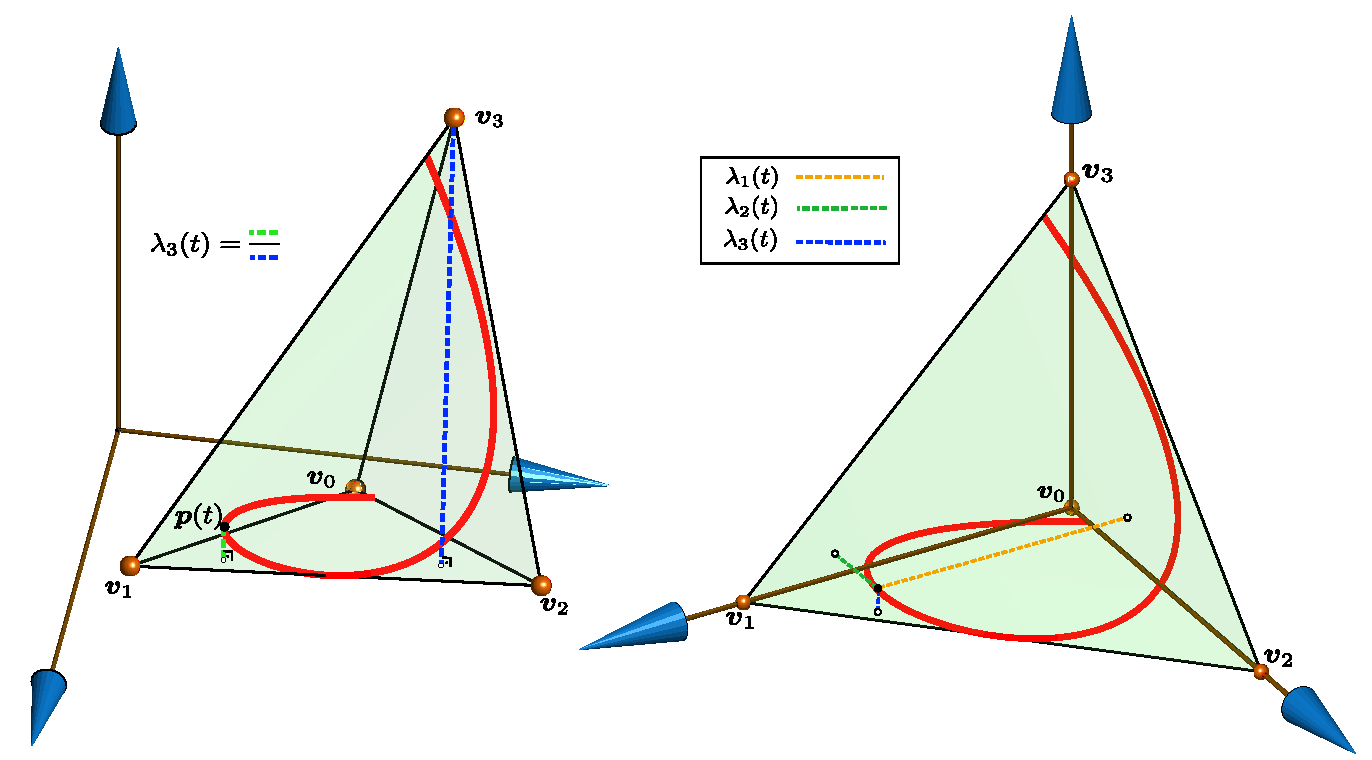
\includegraphics[width=1\columnwidth]{src/imgs/geom_meaning_lambdai_modified}
\par\end{centering}
\caption{Geometric interpretation of $\lambda_{i}(t)$. Each $\lambda_{i}(t)$
represents the distance between the vertex $\boldsymbol{v}_{i}$ and
the plane formed by the vertexes $\boldsymbol{v}_{i}\;\;i\protect\neq j$,
normalized with the distance from $\boldsymbol{v}_{i}$ to that plane
(left). For a standard simplex in 3D (right), the curve in red is
$\boldsymbol{p}(t)=\left[\protect\begin{array}{ccc}
\lambda_{1}(t) & \lambda_{2}(t) & \lambda_{3}(t)\protect\end{array}\right]^{T}$.\label{fig:Geometric-interpretation-of}}

\vskip-2ex
\end{figure}

Finally note that the second constraint can be rewritten as $\boldsymbol{A}^{T}\boldsymbol{1}=\boldsymbol{e}$
(or equivalently $\boldsymbol{e}^{T}\boldsymbol{A}^{-1}=\boldsymbol{1}^{T}$).

\subsection{Objective Function of Problem 1}

Given the previous relationships, note that, 

\[
\left|\left[\begin{array}{cc}
\boldsymbol{V}^{T} & \boldsymbol{1}\end{array}\right]\right|=\left|\left[\begin{array}{cc}
\boldsymbol{A}^{-T}\boldsymbol{P}^{T} & \boldsymbol{1}\end{array}\right]\right|=
\]

\[
=\left|\boldsymbol{A}^{-T}\right|\left|\left[\begin{array}{c}
\boldsymbol{P}^{T}\underbrace{\boldsymbol{A}^{T}\boldsymbol{1}}_{=\boldsymbol{e}^{T}}\end{array}\right]\right|\propto\left|\boldsymbol{A}^{-1}\right|=\frac{1}{|\boldsymbol{A}|}
\]

where in the last step we have used the fact that everything inside
the second determinant is given (i.e. not a decision variable of the
optimization problem), and the fact that $\left|\boldsymbol{A}\right|=\left|\boldsymbol{A}^{T}\right|$.
Therefore, we conclude that $f_{1}\propto\frac{1}{abs\left(|\boldsymbol{A}|\right)}$.
We can therefore maximize $abs(\left|\boldsymbol{A}\right|)$, or,
equivalently, minimize $-abs\left(\left|\boldsymbol{A}\right|\right)$.

\subsection{Objective Function of Problem 2}

Similarly to the previous subsection, we have that

\[
\left|\left[\begin{array}{c}
\boldsymbol{P}\\
\boldsymbol{e}^{T}
\end{array}\right]\right|=\left|\left[\begin{array}{c}
\boldsymbol{V}\\
\underbrace{\boldsymbol{e}^{T}\boldsymbol{A}^{-1}}_{=\boldsymbol{1}^{T}}
\end{array}\right]\boldsymbol{A}\right|\propto\left|\boldsymbol{A}\right|
\]

And therefore, $f_{2}\propto-abs\left(\left|\boldsymbol{A}\right|\right)$

\subsection{Equivalent Formulation for problem 1 and 2}

Therefore, we can solve problem 1 (or problem 2 respectively) for
\textbf{any} given polynomial curve (any given simplex) by solving
the following problem: 

\vspace{0.2cm}

\noindent\fcolorbox{black}{problem3_color}{\begin{minipage}[t]{1\columnwidth - 2\fboxsep - 2\fboxrule}%

\textbf{Problem 3: }

\[
\min_{\boldsymbol{A}}\quad f_{3}:=-abs\left(\left|\boldsymbol{A}\right|\right)
\]

\[
\begin{array}{cc}
s.t. & \boldsymbol{A}\boldsymbol{t}\ge\boldsymbol{0}\quad\forall t\in[-1,1]\\
 & \boldsymbol{A}^{T}\boldsymbol{1}=\boldsymbol{e}
\end{array}
\]

%
\end{minipage}}

\vspace{0.2cm}

Note that Problem 3 is nonconvex, since the objective function is
the determinant of a non-symmetric matrix. 

We can use now Sum-Of-Squares programming, which is an \emph{if and
only if }condition for univariate polynomials to rewrite the second
constraint of problem 2 \cite{Parrilo09}:
\begin{itemize}
\item If $n$ is odd, $\lambda_{i}(t)\ge0\;\;\forall t\in[-1,1]$ if and
only if
\end{itemize}
\[
\left\{ \begin{array}{c}
\lambda_{i}(t)=\hat{\boldsymbol{t}}^{T}\left((t+1)\boldsymbol{W}_{i}+(1-t)\boldsymbol{V}_{i}\right)\hat{\boldsymbol{t}}\\
\boldsymbol{W}_{i}\in\mathbb{S}_{+}^{\frac{n+1}{2}},\boldsymbol{V}_{i}\in\mathbb{S}_{+}^{\frac{n+1}{2}}
\end{array}\right.
\]

\begin{itemize}
\item If $n$ is even, $\lambda_{i}(t)\ge0\;\;\forall t\in[-1,1]$ if and
only if
\end{itemize}
\[
\left\{ \begin{array}{c}
\lambda_{i}(t)=\hat{\boldsymbol{t}}^{T}\boldsymbol{W}_{i}\hat{\boldsymbol{t}}+\hat{\boldsymbol{t}}^{T}(t+1)(1-t)\boldsymbol{V}_{i}\hat{\boldsymbol{t}}\\
\boldsymbol{W}_{i}\in\mathbb{S}_{+}^{\frac{n}{2}+1},\boldsymbol{V}_{i}\in\mathbb{S}_{+}^{\frac{n}{2}}
\end{array}\right.
\]

Note that the \emph{if and only if} condition applies because it is
a univariate polynomial \cite{Parrilo09}. We end up therefore with
a nonconvex finite-dimensional optimization problem, where the decision
variables are the positive semidefinite matrices $\boldsymbol{W}_{i}$
and $\boldsymbol{V}_{i}$, $i\in[0,n]$. 

No generality has been lost in problem 3. However, one disadvantage
is that it easily becomes intractable for larger $n$. To make it
more tractable, we can try to reduce the number of decision variables
of Problem 4 by imposing an structure in $\lambda_{i}(t)$. As Problem
1 is trying to minimize the volume of the simplex, we can impose that
the planes of the $n$-simplex be tangent to the curve \cite{zhou2002algorithms,klee1986facet}.
Using the geometric interpretation of these $\lambda_{i}(t)$ given
in subsection \ref{subsec:Constraints-of-Problem}, this means that
each $\lambda_{i}(t)$ should have either real double roots (places
where the curve is tangent to the plane), and/or roots at $t=\pm1$.
This translates into the formulation shown in Problem 4.

\vspace{0.2cm}

\begin{figure}
\noindent\fcolorbox{black}{problem4_color}{\begin{minipage}[t]{1\columnwidth - 2\fboxsep - 2\fboxrule}%

\textbf{Problem 4:}

\[
\min_{\boldsymbol{A}}\quad f_{4}:=-abs\left(\left|\boldsymbol{A}\right|\right)
\]

\[
s.t:
\]

\textbf{\uline{If \mbox{$n$} is odd:}}

\[
\begin{array}{c}
\lambda_{i}(t)=-b_{i}(t-1)\stackrel[j=1]{\frac{n-1}{2}}{\prod}(t-t_{j})^{2}\quad i=0,2,...,n-1\\
\lambda_{i}(t)=\lambda_{n-i+2}(-t)\quad\quad\quad i=1,3,...,n\\
b_{i}\ge0\quad i=0,2,...,n-1\\
\sum_{i=0}^{i=n}\lambda_{i}(t)=1
\end{array}
\]

\textbf{\uline{If \mbox{$n$} is even:}} define $\mathcal{I}_{a}$
the set of odd integers $\in\left[0,\frac{n}{2}-1\right]$, and $\mathcal{I}_{b}$
the set of even integers $\in\left[0,\frac{n}{2}-1\right]$: 

\[
\begin{array}{c}
\lambda_{i}(t)=-b_{i}(t+1)(t-1)\stackrel[j=1]{\frac{n-2}{2}}{\prod}(t-t_{j})^{2}\quad i\in\mathcal{I}_{a}\\
\lambda_{i}(t)=b_{i}\stackrel[j=1]{\frac{n}{2}}{\prod}(t-t_{j})^{2}\quad\quad\quad i\in\mathcal{I}_{b}\\
\lambda_{j}(t)=\lambda_{n-i+1}(-t)\quad\quad\quad i=\frac{n}{2}+1,...,n\\
b_{i}\ge0\quad i\le\frac{n}{2}\\
\sum_{i=0}^{i=n}\lambda_{i}(t)=1
\end{array}
\]

\begin{itemize}
\item If $\frac{n}{2}$ is odd ($n=2,6,10...)$:
\end{itemize}
\[
\lambda_{i}(t)=-b_{i}(t+1)(t-1)\stackrel[j=1]{\frac{n-2}{4}}{\prod}(t-t_{j})^{2}(t+t_{j})^{2}\quad\quad i=\frac{n}{2}
\]

\begin{itemize}
\item If $\frac{n}{2}$ is even ($n=4,8,12...)$:
\end{itemize}
\[
\lambda_{i}(t)=b_{i}\stackrel[j=1]{\frac{n}{4}}{\prod}(t-t_{j})^{2}(t+t_{j})^{2}\quad\quad i=\frac{n}{2}
\]

%
\end{minipage}}
\end{figure}

The relationship between Problems 1, 2, 3 and 4 is given in Fig. \ref{fig:relationships_problems}.
First note that the structure imposed for the $\lambda_{i}(t)$ in
Problem 4 guarantees that they are nonnegative for $t\in[-1,1]$.
Hence the feasible set of Problem 4 is contained in the feasible set
of Problem 3 or, in other words, any feasible solution of Problem
4 is feasible for Problem 3 (the converse is not true in general).
Therefore, $f_{3}^{*}\le f_{4}^{*}$ holds. The matrix $\boldsymbol{A}^{*}$
found in Problem 3 or 4 can be used to find the vertexes of the simplex
in Problem 1 (by simply using $\boldsymbol{V}^{*}=\boldsymbol{P}\left(\boldsymbol{A}^{*}\right)^{-1}$
where $\boldsymbol{P}$ is the coefficient matrix of the polynomial
given), or to find the polynomial matrix in Problem 2 (by using $\boldsymbol{P}^{*}=\boldsymbol{V}\boldsymbol{A}^{*}$,
where $\boldsymbol{V}$ contains the vertexes of the simplex given).

\begin{figure}
\begin{centering}
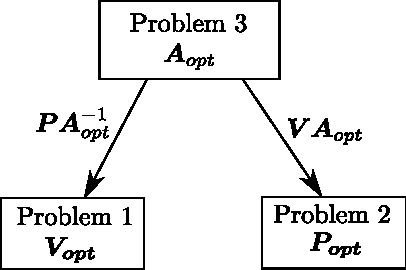
\includegraphics[width=1\columnwidth]{src/imgs/relationships_problems}
\par\end{centering}
\caption{Relationship between Problems 1, 2, 3 and 4: Problem 4 and Problem
3 have the same objective function, but the feasible set of Problem
4 is contained in the feasible set of Problem 3, and therefore $f_{3}^{*}\le f_{4}^{*}$.
Both Problem 3 and 4 generate a (potentially locally) optimal solution
$\boldsymbol{A}^{*}$, which can be applied to any polynomial curve
to find the simplex in Problem 1, or to any simplex to find the polynomial
curve in Problem 2. \label{fig:relationships_problems}}

\vskip-2ex
\end{figure}

\vspace{0.2cm}


\section{Results}

The optimization Problems 2 and 3 have been solved using the nonconvex
solvers IPOPT \cite{wachter2006implementation} and Knitro \cite{byrd2006k,byrd1999interior}
(for Problem 3), the fmincon nonconvex solver \cite{matlabOptToolbox}
(for Problem 4), and the Yalmip \cite{Lofberg2004} interface. 

We were able to find local minima for Problem 4 for $n=1,2,3,4,5,6,7$,
and the same local minima were found in Problem 3 for $n=1,2,3,4$
(Problem 3 becomes intractable for higher $n$). The optimal matrices
$\boldsymbol{A}$ found are shown in Table \ref{tab:table_matrices}.
Note that any permutation in the rows of A will also be a minimizer
(since only the sign of the determinant is affected).

The corresponding plots of the basis functions are shown in Fig. \ref{fig:minvo_and_bernstein},
together with the Bernstein basis and the Lagrange basis for comparison. 

One natural question to ask is whether the basis found constitutes
a global minimizer either for Problem 3 or Problem 4. To answer this,
first note that both Problem 3 and Problem 4 are polynomial optimization
problems. Therefore, we can make use of Lasserre's moment method \cite{lasserre2001},
and increase the order of the moment relaxation to find tighter lower
bounds of the original nonconvex polynomial optimization problem.
Using this technique, we were able to obtain the same objective value
(proving therefore global optimality) for $n=1,2,3,4$ (in Problem
4), and for $n=1$ (in Problem 3). 

These results lead us to the following conclusions (also summarized
in Table \ref{tab:table_matrices}):
\begin{itemize}
\item The matrix $\boldsymbol{A}$ found for $n=1$ is a global minimizer
of both Problem 3 and Problem 4.
\item The matrices $\boldsymbol{A}$ found for $n=2,3,4$ are global minimizers
for Problem 4, and at least local minimizers for Problem 3.
\item The matrices $\boldsymbol{A}$ found for $n=5,6,7$ are at least local
minimizers for Problem 4, and are at least feasible solutions for
Problem 3.
\end{itemize}
In Table \ref{tab:table_matrices}, it is also shown the ratio 

\[
\frac{abs\left(|\boldsymbol{A}_{B}|\right)}{abs\left(|\boldsymbol{A}|\right)}
\]

, where $\boldsymbol{A}$ and $\boldsymbol{A}_{B}$ denote the associated
matrices for the MINVO and Bernstein basis respectively. 

Let us know analyze the meaning of these results in both for the Problems
1 and 2. 

\subsection{From the point of view of Problem 1}

Problem 1 attempts to find the simplex with smallest volume the encloses
a given polynomial curve. In Fig. \ref{fig:comparison2d} it is shown
the simplex found for $n=2$, and in Fig. \ref{fig:Comparison3d}
and for $n=3$. The simplex found using the Bernstein basis is also
shown for comparison. Let $S$ and $S_{B}$ denote the simpleces that
the MINVO and Bernstein basis generate respectively, we have that:

\[
\frac{vol\left(S\right)}{vol\left(S_{B}\right)}=\frac{abs\left(|\boldsymbol{A}_{B}|\right)}{abs\left(|\boldsymbol{A}|\right)}
\]

This means, for instance, that for $n=3$, the MINVO basis finds a
simplex that is $\approx2.36$ smaller than the one the Bernstein
basis finds. For $n=7$, the MINVO basis is able to obtain a simplex
that is $\approx903$ times\textbf{ }smaller than the one achieved
using the Bernstein basis. 

\subsection{From the point of view of Problem 2}

In problem 2, the $n$-simplex $S$ is given, and we obtain the polynomial
curve that is contained in $S$, whose coefficients vectors $\boldsymbol{p}_{n},...,\boldsymbol{p}_{1}$
span a parallelogram with largest volume. The results for a regular
triangle and a tetrahedron ($n=2$ and $n=3$) are shown in Figs.
\ref{fig:comparison2d_simplex_given} and \ref{fig:comparison3d_simplex_given}
respectively). Similar to the previous case, let $P$ and $P_{B}$
denote the parallelograms that the MINVO and Bernstein basis generate
respectively, we have that:

\[
\frac{vol\left(P_{B}\right)}{vol\left(P\right)}=\frac{abs\left(|\boldsymbol{A}_{B}|\right)}{abs\left(|\boldsymbol{A}|\right)}
\]

which means that, for $n=3$, the MINVO basis finds a parallelogram
$\approx2.36$ times bigger than the Bernstein basis ($\approx903$
times bigger for $n=7$). 

\begin{figure}
\begin{centering}
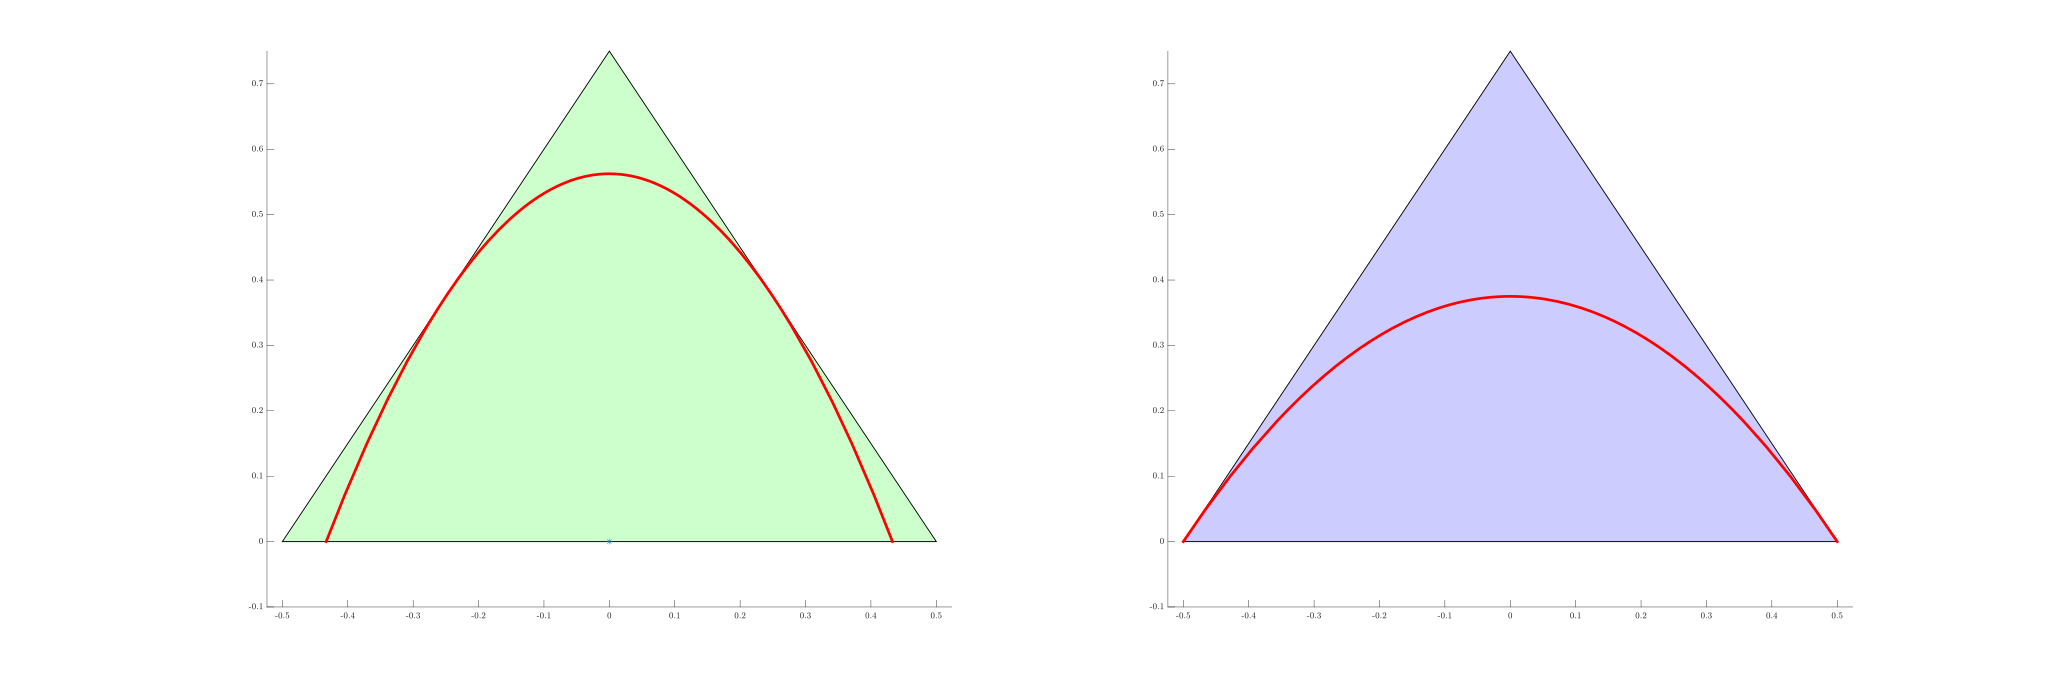
\includegraphics[width=1\columnwidth]{src/imgs/comparison2d_simplex_given}
\par\end{centering}
\caption{Optimal solution for Problem 2 with $n=2$. The triangle is given,
and the red polynomial curve using the MINVO basis is the one whose
coefficients vectors $\boldsymbol{p}_{2},\boldsymbol{p}_{1}$ span
a rectangle with largest area, while being contained in the triangle.
On the right, the curve obtained using the Bernstein basis. \label{fig:comparison2d_simplex_given} }

\vskip-2ex
\end{figure}

\begin{figure}
\begin{centering}
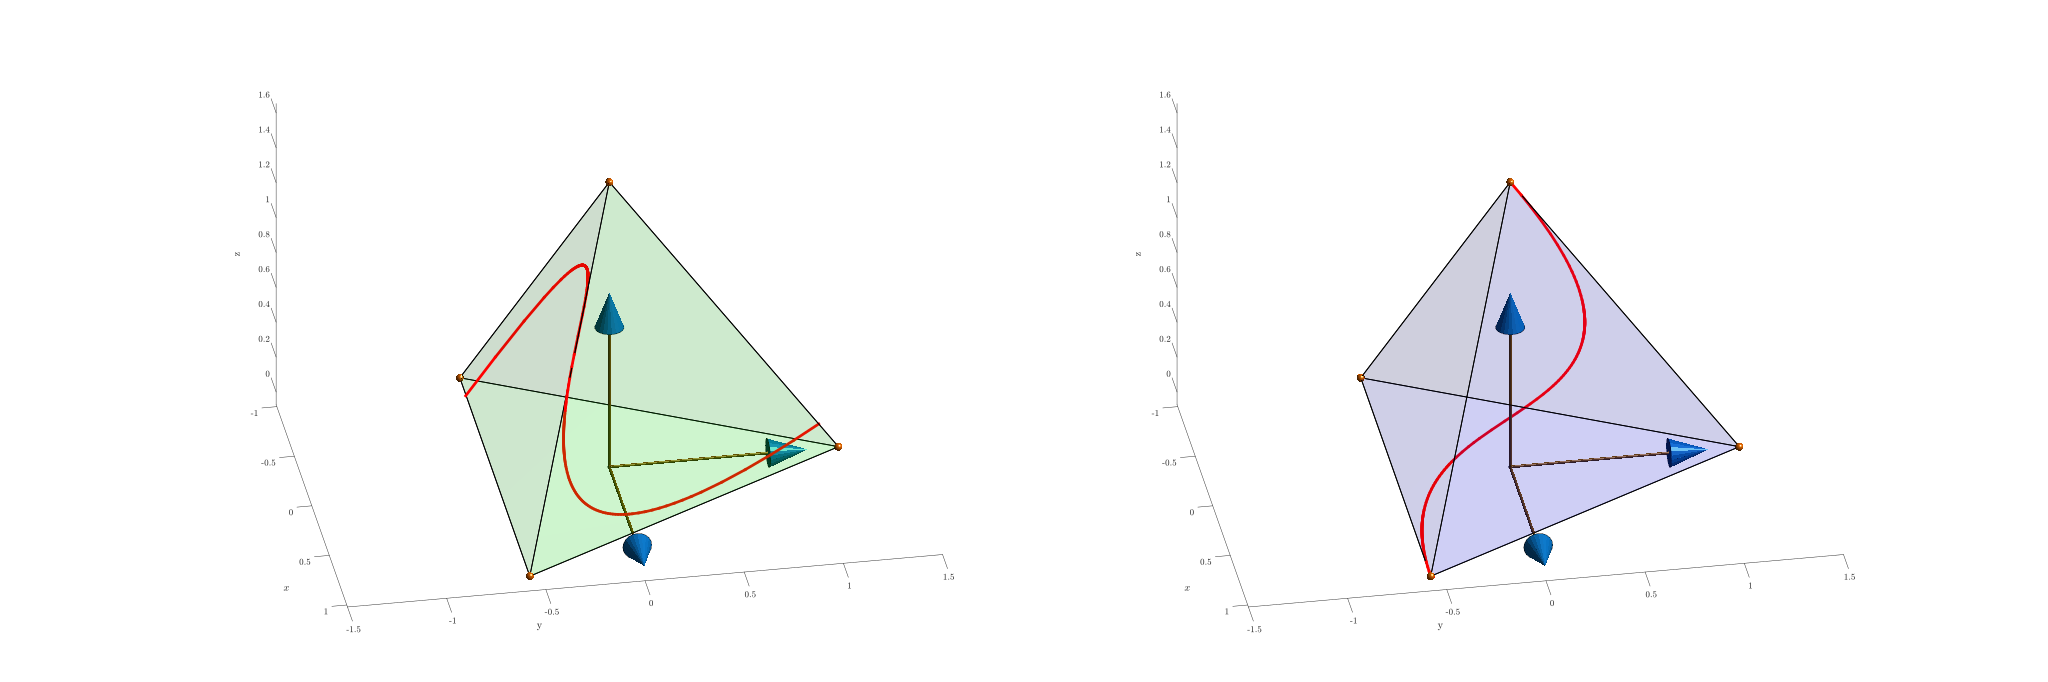
\includegraphics[width=1\columnwidth]{src/imgs/comparison3d_simplex_given}
\par\end{centering}
\caption{Optimal solution for Problem 2 with $n=3$. The tetrahedron is given,
and the red polynomial curve using the MINVO basis is the curve inside
the tetrahedron whose coefficients vectors $\boldsymbol{p}_{3},\boldsymbol{p}_{2},\boldsymbol{p}_{1}$
span a paralellogram with largest volume. On the right, the curve
obtained using the Bernstein basis. \label{fig:comparison3d_simplex_given}}

\vskip-2ex
\end{figure}

\begin{figure}
\begin{centering}

\includegraphics[width=0.8\columnwidth]{src/imgs/comparison2d}
\par\end{centering}
\caption{Comparison between the MINVO basis and the Bernstein basis for $n=2$.
The simplex found using the MINVO basis (left) encloses the $2^{nd}$-order
polynomial curve in red, and, for any $2^{nd}$-order polynomial curve,
the MINVO basis generates a simplex that is $\approx1.3$ times smaller
that the one found using the Bernstein basis (right). \label{fig:comparison2d}}

\vskip-2ex
\end{figure}

{\setlength\extrarowheight{1pt}
 \setlength\tabcolsep{0pt}
%\renewcommand{\arraystretch}{1.}

\begin{table*}
\begin{centering}
\begin{tabular}{|c|c|c|c|>{\columncolor{problem3_color}\centering}c|>{\columncolor{problem4_color}\centering}c|}
\hline 
\textbf{\hspace{0.1cm}$\boldsymbol{n}$ } & $\boldsymbol{A}$ & $abs\left(\left|\boldsymbol{A}\right|\right)$ & $\frac{abs\left(|\boldsymbol{A}_{B}|\right)}{abs\left(|\boldsymbol{A}|\right)}$ & \textbf{Problem 3} & \textbf{Problem 4}\tabularnewline
\hline 
\hline 
$1$ & {\scriptsize{}$\frac{1}{2}\left[\begin{array}{cc}
-1 & 1\\
1 & 1
\end{array}\right]$} & $\frac{1}{2}=0.5$ & $=1$ & Global Opt. & Global Opt.\tabularnewline
\hline 
$2$ & {\scriptsize{}$\frac{1}{8}\left[\begin{array}{ccc}
3 & -2\sqrt{3} & 1\\
-6 & 0 & 6\\
3 & 2\sqrt{3} & 1
\end{array}\right]$} & $\frac{3\sqrt{3}}{16}\approx0.3248$ & $\approx0.7697$ & $\begin{array}{c}
\text{Local Opt.}\\
\text{(at least)}
\end{array}$ & Global Opt.\tabularnewline
\hline 
$3$ & {\scriptsize{}$\left[\begin{array}{cccc}
-0.4302 & 0.4568 & -0.02698 & 0.0004103\\
0.8349 & -0.4568 & -0.7921 & 0.4996\\
-0.8349 & -0.4568 & 0.7921 & 0.4996\\
0.4302 & 0.4568 & 0.02698 & 0.0004103
\end{array}\right]$} & $\approx0.3319$ & $\approx0.4237$ & $\begin{array}{c}
\text{Local Opt.}\\
\text{(at least)}
\end{array}$ & Global Opt.\tabularnewline
\hline 
$4$ & {\scriptsize{}$\left[\begin{array}{ccccc}
-1.108 & -0.8108 & 0.9602 & 0.8108 & 0.1483\\
-1.108 & 0.8108 & 0.9602 & -0.8108 & 0.1483\\
0.5255 & -0.5758 & -0.09435 & 0.1381 & 0.03023\\
0.5255 & 0.5758 & -0.09435 & -0.1381 & 0.03023\\
1.166 & 0 & -1.732 & 0 & 0.643
\end{array}\right]$} & $\approx0.5678$ & $\approx0.1651$ & $\begin{array}{c}
\text{Local Opt.}\\
\text{(at least)}
\end{array}$ & $\begin{array}{c}
\text{Local Opt.}\\
\text{(at least)}
\end{array}$\tabularnewline
\hline 
$5$ & {\scriptsize{}$\left[\begin{array}{cccccc}
-0.7392 & 0.7769 & 0.3302 & -0.3773 & -0.0365 & 0.04589\\
1.503 & -1.319 & -1.366 & 1.333 & -0.121 & 0.002895\\
-1.75 & 0.5424 & 2.777 & -0.9557 & -1.064 & 0.4512\\
1.75 & 0.5424 & -2.777 & -0.9557 & 1.064 & 0.4512\\
-1.503 & -1.319 & 1.366 & 1.333 & 0.121 & 0.002895\\
0.7392 & 0.7769 & -0.3302 & -0.3773 & 0.0365 & 0.04589
\end{array}\right]$} & $\approx1.6987$ & $\approx0.0449$ & $\begin{array}{c}
\text{Feasible}\\
\text{(at least)}
\end{array}$ & $\begin{array}{c}
\text{Local Opt.}\\
\text{(at least)}
\end{array}$\tabularnewline
\hline 
$6$ & {\scriptsize{}$\left[\begin{array}{ccccccc}
1.06 & -1.134 & -0.7357 & 0.8348 & 0.1053 & -0.1368 & 0.01836\\
-2.227 & 2.055 & 2.281 & -2.299 & -0.08426 & 0.2433 & 0.0312\\
2.59 & -1.408 & -4.27 & 2.468 & 1.58 & -1.081 & 0.152\\
-2.844 & 0 & 5.45 & 0 & -3.203 & 0 & 0.5969\\
2.59 & 1.408 & -4.27 & -2.468 & 1.58 & 1.081 & 0.152\\
-2.227 & -2.055 & 2.281 & 2.299 & -0.08426 & -0.2433 & 0.0312\\
1.06 & 1.134 & -0.7357 & -0.8348 & 0.1053 & 0.1368 & 0.01836
\end{array}\right]$} & $\approx9.1027$ & $\approx0.00848$ & $\begin{array}{c}
\text{Feasible}\\
\text{(at least)}
\end{array}$ & $\begin{array}{c}
\text{Local Opt.}\\
\text{(at least)}
\end{array}$\tabularnewline
\hline 
$7$ & {\scriptsize{}$\left[\begin{array}{cccccccc}
-1.637 & 1.707 & 1.563 & -1.682 & -0.3586 & 0.4143 & -0.006851 & 2.854\cdot10^{-5}\\
3.343 & -3.285 & -3.947 & 4.173 & 0.6343 & -0.9385 & -0.02111 & 0.05961\\
-4.053 & 2.722 & 6.935 & -4.96 & -2.706 & 2.269 & -0.2129 & 0.00535\\
4.478 & -1.144 & -9.462 & 2.469 & 6.311 & -1.745 & -1.312 & 0.435\\
-4.478 & -1.144 & 9.462 & 2.469 & -6.311 & -1.745 & 1.312 & 0.435\\
4.053 & 2.722 & -6.935 & -4.96 & 2.706 & 2.269 & 0.2129 & 0.00535\\
-3.343 & -3.285 & 3.947 & 4.173 & -0.6343 & -0.9385 & 0.02111 & 0.05961\\
1.637 & 1.707 & -1.563 & -1.682 & 0.3586 & 0.4143 & 0.006851 & 2.854\cdot10^{-5}
\end{array}\right]$} & $\approx89.0191$ & $\approx0.00110$ & $\begin{array}{c}
\text{Feasible}\\
\text{(at least)}
\end{array}$ & $\begin{array}{c}
\text{Local Opt.}\\
\text{(at least)}
\end{array}$\tabularnewline
\hline 
\end{tabular}\textbf{ }
\par\end{centering}

\caption{Results for the MINVO basis. $\boldsymbol{A}$ denotes the coefficient
matrix of the MINVO basis (i.e. each polynomial in the basis is given
by the rows of $\boldsymbol{A}\boldsymbol{t}$), while $\boldsymbol{A}_{B}$
represents the matrix of the Bernstein basis ($t\in[-1,1]$ for both).
The bigger the absolute value of the determinant, the smaller the
associated simplex (for Problem 1) and the smaller the parallelogram
(for Problem 3). These matrices $\boldsymbol{A}$ are independent
of the polynomial curve given (in Problem 1), or of the simplex given
(in Problem 2). \label{tab:table_matrices}}
\end{table*}

}

\begin{figure*}
\begin{centering}
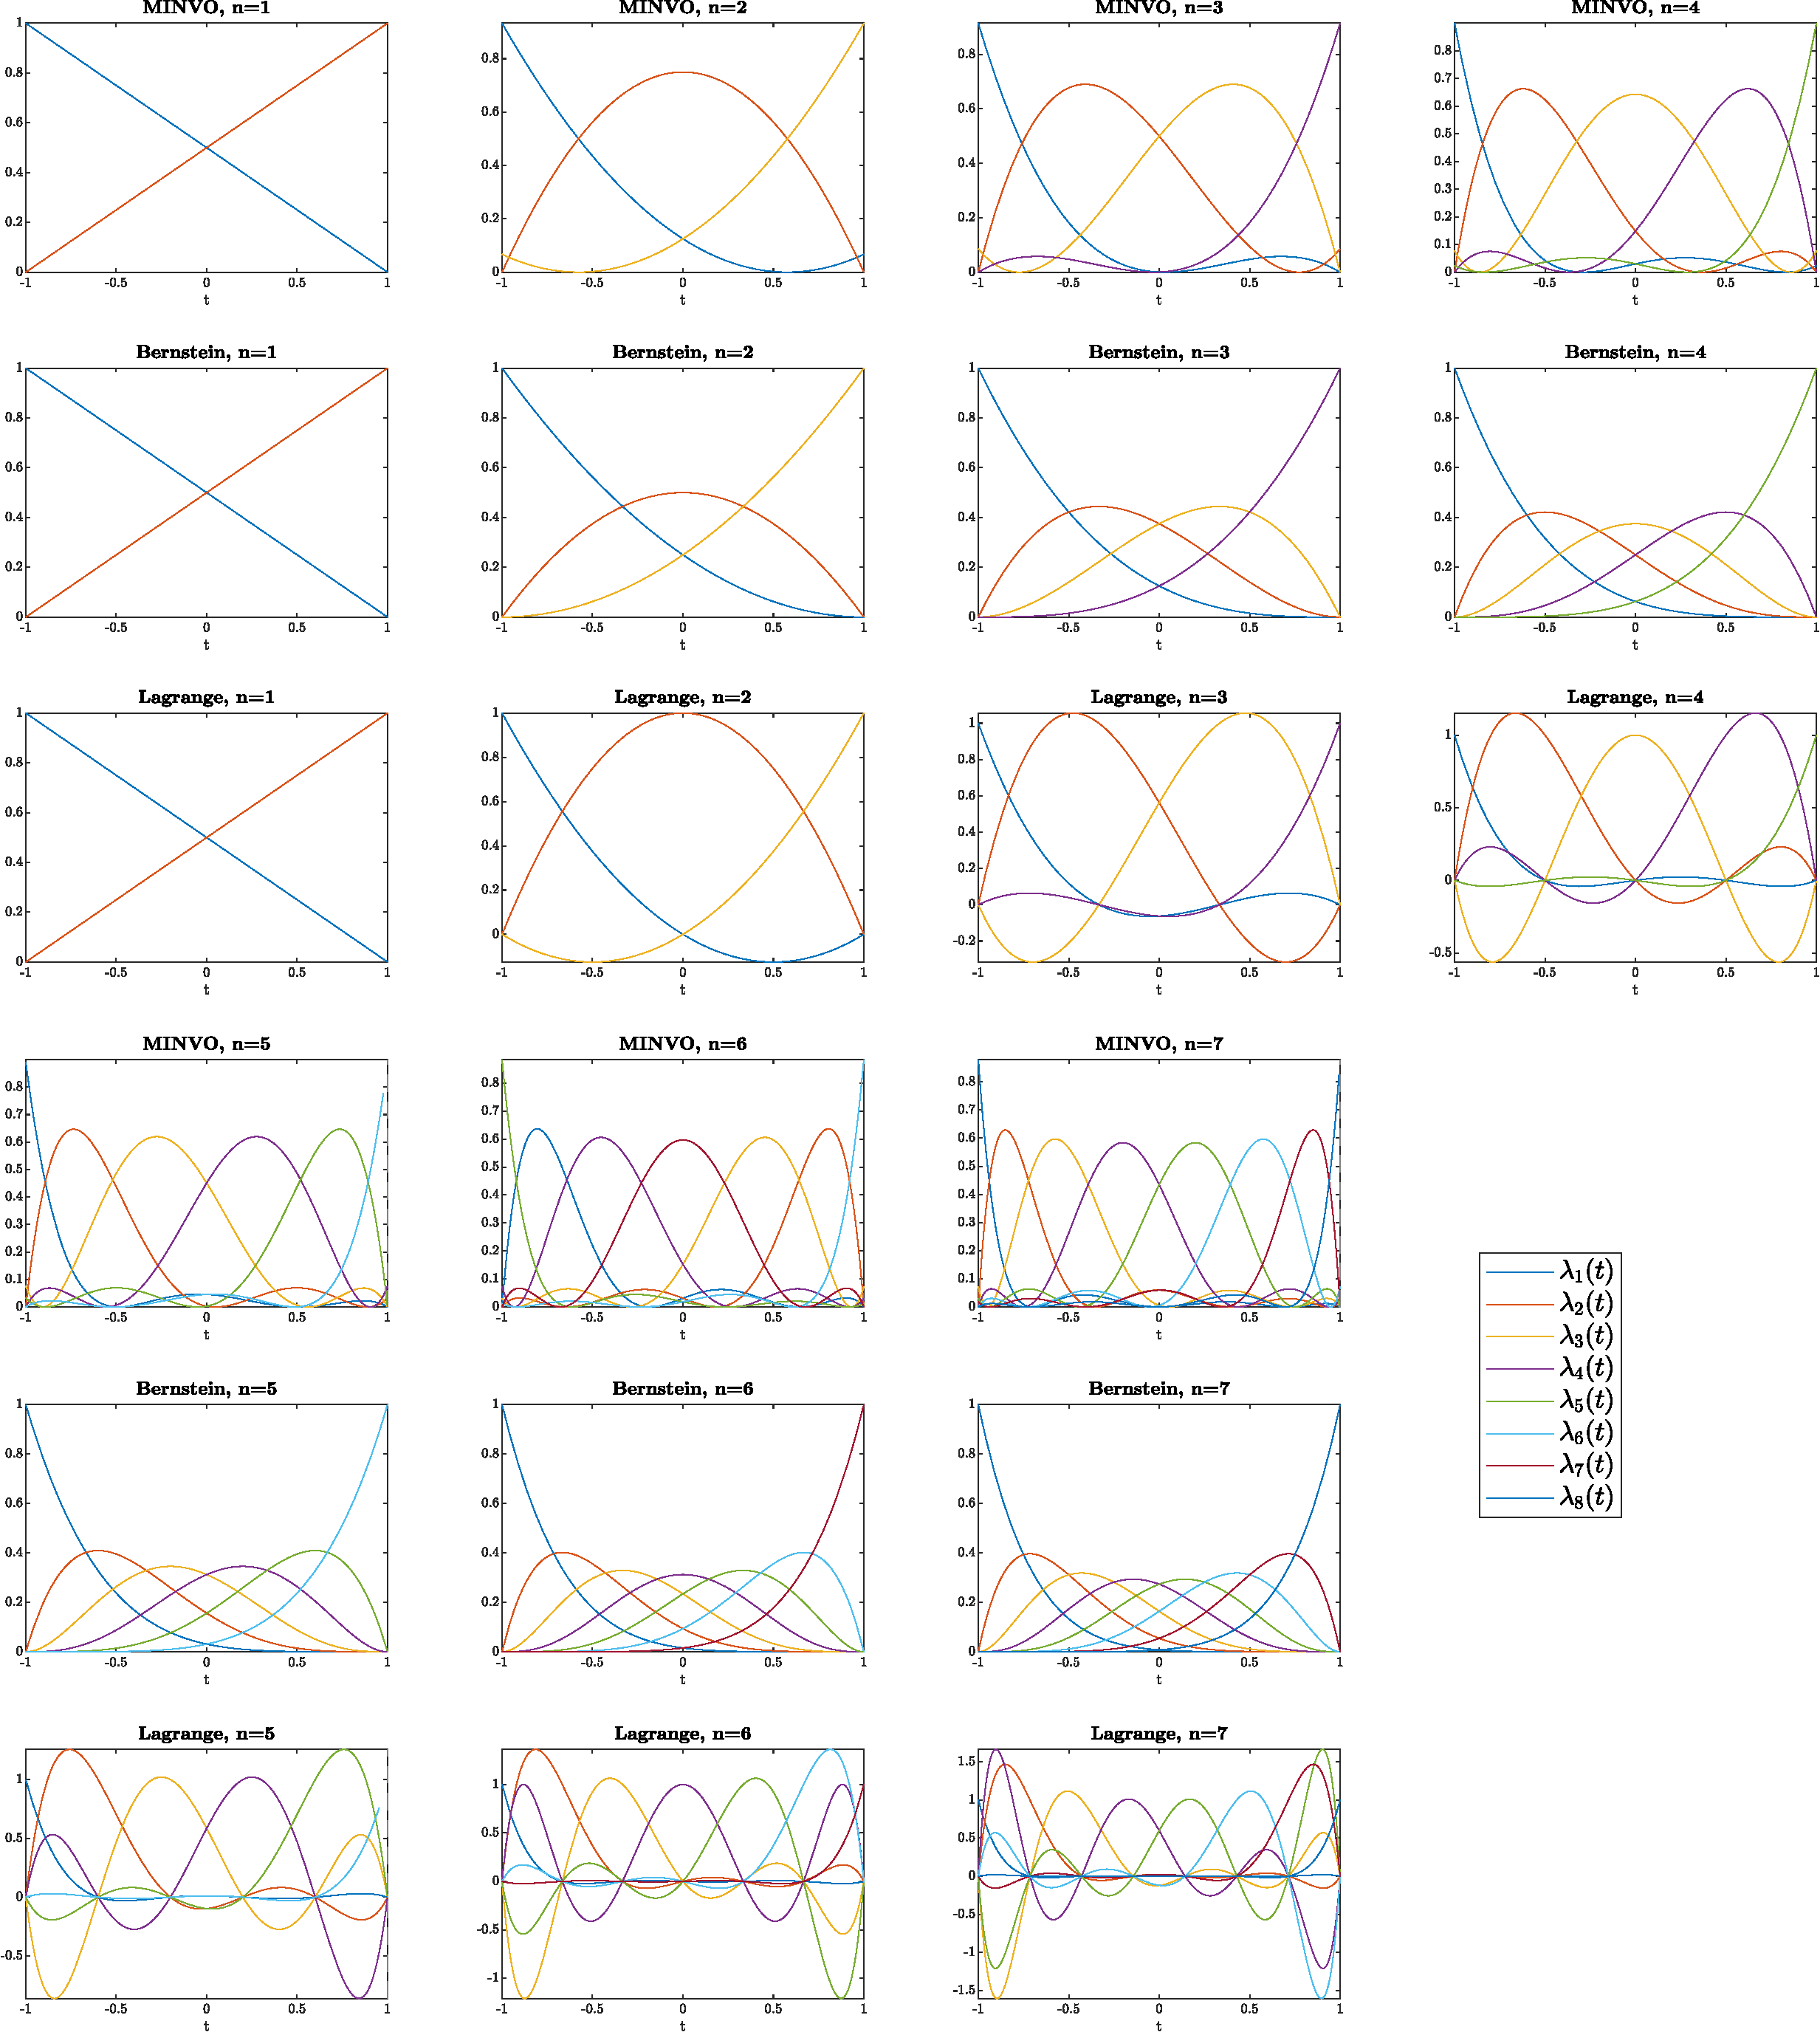
\includegraphics[width=1\textwidth]{src/imgs/plots_basis}
\par\end{centering}
\caption{Comparison between the MINVO, Lagrange and Bernstein basis for $n=1,2,3,4,5,6,7$.
All these basis satisfy $\sum_{i=0}^{i=n}\lambda_{i}(t)=1$, and the
MINVO and Bernstein basis also satisfy $\lambda_{i}(t)\ge0\;\forall t\in[-1,1]$
\label{fig:minvo_and_bernstein}}

\vskip-2ex
\end{figure*}


\section{Conclusions and Future Work}

This work derived and presented the MINVO basis. The key features
of this basis is that it finds the smallest $n$-simplex that encloses
a given polynomial curve (Problem 1), and also finds the polynomial
curve that is inside a given simplex, and whose coefficient vectors
$\boldsymbol{p}_{n},...,\boldsymbol{p}_{1}$ generate a parallelogram
with largest volume (Problem 2). Global Optimality was also proven
for some $n$.

The exciting results of this project naturally lead to the following
questions and conjectures:
\begin{itemize}
\item Is the global optimum of Problem 3 the same as the global optimum
of Problem 4? In other words, are we losing generality by imposing
the specific structure in $\lambda_{i}(t)$?. The results seem to
indicate that it is likely that no generality is lost. 
\item Does there exist an analytical solution (i.e. not numerical) for Problem
3 for any degree $n$? 
\item Does there exist a recursivity formula to obtain the solution of problem
3 for $n$ given the previous solutions $1,...,n-1$? Would this recursivity
formula allow to easily prove global optimality for all $n$ of Problem
3?
\end{itemize}

\section{Acknowledgements}

The author would like to thank Prof. Gilbert Strang, Prof. Jonathan
How, Prof. Johan L�fberg, Ashkan M. Jasour, Kasra Khosoussi, Juan
Jos� Madrigal and Marc Adill�n for helpul insights and discussions. 

\selectlanguage{english}%
\bibliographystyle{unsrt}
\addcontentsline{toc}{section}{\refname}\bibliography{bibliography}

\selectlanguage{american}%

\begin{center}
\par\end{center}


\end{document}
